\documentclass{article}

\usepackage{pythontex}
\usepackage{graphicx}

\usepackage{url}

\begin{document}

\section{Creating a chart}
\begin{pycode}
from matplotlib import pyplot as plt
import numpy as np
plt.rc('text', usetex=True)
plt.rc('font', family='serif')
plt.rc('font', size=10.0)
plt.rc('legend', fontsize=10.0)
plt.rc('font', weight='normal')

x = np.linspace(0, 30)
y = values = np.random.randint(0, 20, size=50)

z = np.sin(x)+np.cos(x/2) + y

plt.figure(figsize=(4, 2.5))
plt.plot(x, z, label='$\sin(x) + cos(x/2) + y$')

plt.xlabel(r'$x\mathrm{-axis}$')
plt.ylabel(r'$y\mathrm{-axis}$')
plt.legend(loc='lower right')
plt.savefig('myplot.pdf', bbox_inches='tight')
\end{pycode}

\begin{center}
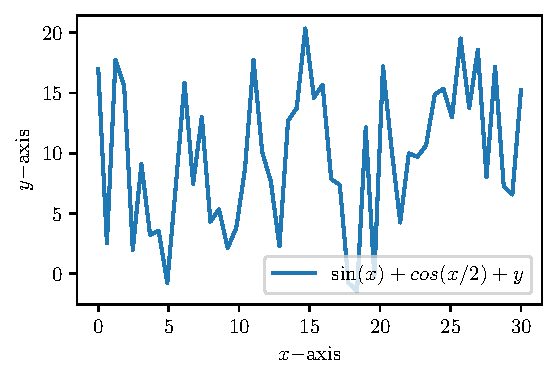
\includegraphics{myplot.pdf}
\end{center}


\begin{pycode}
from datetime import date

from openpyxl import Workbook
from openpyxl.chart import LineChart,Reference
from openpyxl.chart.axis import DateAxis

wb = Workbook()
ws = wb.active

for idx, (a, b) in enumerate(zip(x, y), 1):
    ws.append([a, b, f"=SIN(A{idx})+COS(A{idx}/2)+B{idx}"])

c1 = LineChart()

data = Reference(ws, min_col=3,  max_col=3, min_row=1, max_row=len(y))
c1.add_data(data)

ws.add_chart(c1, "D2")

wb.save("chart.xlsx")
\end{pycode}


\section{extract info from changed excel file}

\begin{pycode}
import openpyxl
from prettytable import PrettyTable 

path = "chart_changed.xlsx"
wb = openpyxl.load_workbook(path)
ws = wb.active
print("C\n")
print("----------\n")

for r in ws.iter_rows(values_only=True):
    print(str(r[2])+"\n") 


\end{pycode}


\end{document}
